\documentclass[12pt,a4paper]{article}
\usepackage[left=4cm,right=3cm,top=3cm,bottom=3cm]{geometry}
\usepackage{mathptmx} % Times New Roman
\usepackage[T1]{fontenc}
\usepackage{textcomp}
\usepackage{amsmath}
\usepackage{amssymb}
\usepackage{graphicx}
\usepackage[justification=raggedright,singlelinecheck=false]{caption}
\usepackage{float}
\usepackage{hyperref}
\usepackage[none]{hyphenat}
\usepackage{tikz}
\usepackage{booktabs}
\usepackage{multirow}
\usepackage{enumitem}
\usepackage{varwidth} % Untuk better text wrapping
\usepackage{changepage} % Untuk adjusting margins on specific pages
\usetikzlibrary{shapes.geometric, arrows, positioning, fit, calc, matrix}

% Pengaturan hyphenation - NO HYPHENATION AT ALL
\hyphenpenalty=10000
\exhyphenpenalty=10000
\tolerance=3000 % Increase tolerance
\emergencystretch=10em % Increase emergency stretch
\hyphenchar\font=-1
\sloppy
\hbadness=10000 % Suppress bad hbox warnings
\vbadness=10000 % Suppress bad vbox warnings

% Menghilangkan indentasi paragraf pertama setelah section
\setlength{\parindent}{0pt}
\setlength{\parskip}{6pt}

% Definisi Style TikZ Terpusat
\tikzset{
    block/.style = {rectangle, draw, fill=blue!20, text width=8em, text centered, rounded corners, minimum height=3em},
    io/.style = {ellipse, draw, fill=yellow!20, text width=7em, text centered, minimum height=2em},
    process/.style = {rectangle, draw, fill=green!20, text width=14em, text centered, minimum height=2.5em},
    line/.style = {draw, -latex'},
    skipline/.style = {draw, ->, dashed}
}

\begin{document}

\renewcommand{\thesection}{\Roman{section}}
\renewcommand{\thesubsection}{\thesection.\arabic{subsection}}
\renewcommand{\thesubsubsection}{\thesubsection.\arabic{subsubsection}}
\setcounter{section}{3}
\section{ANALISIS DAN DESAIN}
\label{sec:analisis-desain}

Bab ini menguraikan rancangan solusi teknis yang diusulkan untuk restorasi dokumen terdegradasi dengan pendekatan Generative Adversarial Network yang dimodifikasi secara khusus untuk meningkatkan keterbacaan teks oleh model pengenalan tulisan tangan. Pembahasan dimulai dari analisis kebutuhan sistem (fungsional dan non-fungsional), dilanjutkan dengan rancangan arsitektur solusi yang mencakup desain Generator (U-Net), Recognizer (Transformer-based yang frozen), Diskriminator Dual-Modal (CNN+LSTM), dan fungsi loss multi-komponen (Adversarial + L1 + CTC). Selanjutnya, detail implementasi solusi diuraikan meliputi lingkungan eksperimen, persiapan dataset (ground truth untuk pengenalan tulisan tangan dan sintetis untuk GAN), implementasi arsitektur model dalam TensorFlow/Keras, prosedur training dengan optimasi alternating, dan justifikasi pemilihan hyperparameter melalui studi ablasi.

\subsection{Analisis Kebutuhan Sistem} % This will be numbered as 4.1

Berdasarkan rumusan masalah dan tujuan penelitian, sistem restorasi dokumen yang akan dibangun harus memenuhi serangkaian kebutuhan fungsional dan non-fungsional. Kebutuhan ini menjadi acuan dalam perancangan arsitektur dan tolok ukur dalam evaluasi akhir, sejalan dengan tahapan DSRM.

\subsubsection{Kebutuhan Fungsional} % This will be numbered as 4.1.1 Kebutuhan fungsional mendefinisikan fungsi atau kemampuan spesifik yang harus dimiliki oleh sistem.

Kebutuhan fungsional mendefinisikan fungsi atau kemampuan spesifik yang harus dimiliki oleh sistem GAN-HTR untuk dapat melakukan restorasi dokumen terdegradasi secara efektif. Delapan kebutuhan fungsional yang diidentifikasi mencakup tiga kategori utama:

\begin{enumerate}
    \item Kemampuan Core ML untuk restorasi visual dan pengenalan teks,
    \item Kemampuan Processing untuk menangani batch inference dan dataset sintetis,
    \item Kemampuan System Integration untuk input/output yang terstandar dan antarmuka yang fleksibel.
\end{enumerate}
Setiap kebutuhan dirancang untuk memastikan sistem tidak hanya secara teknis mampu melakukan restorasi, tetapi juga praktis untuk digunakan dalam lingkungan produksi dan dapat diintegrasikan dengan sistem lain.

\begin{table}[htbp!]
\centering
\caption{Ringkasan Functional Requirements Sistem GAN-HTR}
\label{tab:functional_requirements}
\begin{tabular}{p{0.05\textwidth}p{0.20\textwidth}p{0.70\textwidth}}
\toprule
\textbf{Kode} & \textbf{Nama Requirement} & \textbf{Deskripsi dan Detail Spesifikasi} \\
\midrule
FR-1 & Kemampuan Restorasi Gambar & Menerima input gambar dokumen terdegradasi dan menghasilkan output gambar versi restorasi yang lebih bersih secara visual. \\
\midrule
FR-2 & Penanganan Berbagai Jenis Degradasi & Menangani setidaknya 4 jenis degradasi utama: tembusan tinta (*bleed-through*), pemudaran (*fading*), noda (*stains*), dan efek buram (*blur*). \\
\midrule
FR-3 & Integrasi dengan Proses HTR & Gambar hasil restorasi dapat diproses oleh model pengenalan tulisan tangan untuk menghasilkan transkripsi teks. \\
\midrule
FR-4 & Kemampuan Inference Batch Processing & Memproses dokumen terdegradasi ukuran penuh secara batch dengan output: (1) Gambar dokumen restorasi penuh, (2) File transkripsi teks (.txt), (3) File metadata (.json) dengan waktu proses dan confidence scores. \\
\midrule
FR-5 & Dukungan untuk Dataset Sintetis & Menyertakan pipeline untuk pembuatan dataset sintetis terdegradasi dari gambar bersih sebagai mekanisme training utama. \\
\midrule
FR-6 & Output Prediksi Terdefinisi & Menghasilkan output dengan format konsisten: (1) Visual: PNG/TIFF 300 DPI grayscale, (2) Text: UTF-8 dengan confidence score 0.0-1.0 per baris, (3) Quality: PSNR/SSIM, (4) Error: error code dan message. \\
\midrule
FR-7 & Penanganan Input Data Fleksibel & Menangani berbagai kondisi input: (1) Format: JPG, PNG, TIFF, PDF multi-page, (2) Validasi: resolusi minimum 128x1024px, (3) Recovery: skip corrupted files, (4) Preprocessing: konversi grayscale dan noise reduction. \\
\midrule
FR-8 & Kemampuan Integrasi Sistem & Menyediakan antarmuka integrasi: (1) CLI dengan parameter terdefinisi, (2) Python API untuk import aplikasi, (3) Configuration management YAML/JSON, (4) Structured logging interface. \\
\bottomrule
\end{tabular}
\end{table}

\clearpage
\subsubsection{Kebutuhan Non-Fungsional} % This will be numbered as 4.1.2 Kebutuhan non-fungsional mendefinisikan kriteria kualitas atau batasan performa dari sistem.

Kebutuhan non-fungsional mendefinisikan kriteria kualitas atau batasan performa yang harus dipenuhi oleh sistem GAN-HTR. Empat kebutuhan non-fungsional yang ditetapkan mengukur aspek kualitatif dan kuantitatif dari performa sistem, meliputi:

\begin{enumerate}
    \item Kualitas Visual untuk mengukur kesamaan dengan ground truth menggunakan PSNR dan SSIM,
    \item Keterbacaan Teks sebagai metrik utama keberhasilan sistem melalui penurunan CER,
    \item Efisiensi Waktu untuk memastikan kepraktisan penggunaan,
    \item Reproduktifitas untuk menjamin konsistensi dan keandalan hasil eksperimen.
\end{enumerate}
Target performa yang ditetapkan berdasarkan studi literatur dan kebutuhan praktis implementasi di lapangan.

\begin{table}[H]
\centering
\caption{Ringkasan Non-Functional Requirements Sistem GAN-HTR}
\label{tab:non_functional_requirements}
\begin{tabular}{p{0.05\textwidth}p{0.25\textwidth}p{0.65\textwidth}}
\toprule
\textbf{Kode} & \textbf{Nama Requirement} & \textbf{Deskripsi dan Target Performa} \\
\midrule
NFR-1 & Kualitas Visual Restorasi & Kualitas visual gambar hasil restorasi vs ground truth harus mencapai: (1) PSNR rata-rata $\geq$ 35 dB, (2) SSIM rata-rata $\geq$ 0.90 pada dataset validasi. \\
\midrule
NFR-2 & Peningkatan Keterbacaan Teks & Sistem harus meningkatkan akurasi transkripsi HTR secara signifikan: CER menunjukkan penurunan minimal 25\% dibandingkan CER pada gambar terdegradasi asli. \\
\midrule
NFR-3 & Performa Waktu Inferensi & Waktu processing untuk satu gambar dokumen tunggal pada NVIDIA RTX A4000 tidak boleh melebihi 15 detik untuk memastikan kepraktisan penggunaan. \\
\midrule
NFR-4 & Reproduktifitas & Proses training dan evaluasi harus dapat direproduksi dengan lingkungan perangkat lunak dan dependensi yang didefinisikan secara jelas (melalui file \texttt{pyproject.toml}). \\
\bottomrule
\end{tabular}
\end{table}

Berdasarkan Tabel \ref{tab:functional_requirements} dan Tabel \ref{tab:non_functional_requirements}, sistem GAN-HTR yang akan dikembangkan harus memenuhi total 12 kebutuhan (8 fungsional dan 4 non-fungsional) yang mencakup aspek visual, tekstual, performa, dan integrasi sistem.

\subsection{Rancangan Arsitektur} % This will be numbered as 4.2

Rancangan solusi bertujuan untuk membangun sebuah model generatif yang tidak hanya mampu membersihkan gambar dari kerusakan visual, tetapi juga secara eksplisit dioptimalkan untuk menghasilkan gambar yang keterbacaan teksnya maksimal. Untuk mencapai tujuan ini, arsitektur GAN standar dimodifikasi dengan memperkenalkan dua elemen kunci: (1) Diskriminator dual-modal yang menilai koherensi antara gambar dan teks, dan (2) Fungsi loss gabungan yang mencakup loss dari model pengenalan tulisan tangan.

\subsubsection{Gambaran Umum Arsitektur} % This will be numbered as 4.2.1 
Arsitektur yang diusulkan terdiri dari tiga komponen utama yang berinteraksi dalam sebuah kerangka adversarial, seperti yang diilustrasikan pada Gambar \ref{fig:arch_overview}. Ketiga komponen tersebut adalah:
\begin{enumerate}[nosep]
    \item Generator (G): Sebuah model dengan arsitektur U-Net yang bertugas menerima gambar dokumen terdegradasi dan menghasilkan versi restorasi dari gambar tersebut.
    \item Recognizer (R): Sebuah model HTR berbasis Transformer yang sudah terlatih dan dibekukan (frozen). Tujuannya bukan untuk dilatih, melainkan untuk "membaca" teks dari gambar hasil restorasi dan memberikan sinyal loss terkait keterbacaan.
    \item Diskriminator (D): Sebuah model Diskriminator dual-modal yang menjadi inti dari penelitian ini. Tidak seperti diskriminator pada umumnya yang hanya menerima input gambar, diskriminator ini menerima pasangan \textit{(gambar, representasi teks)} untuk menilai apakah sebuah gambar "asli" dan apakah teks di dalamnya koheren.
\end{enumerate}

\begin{figure}[htbp!]
\centering
\resizebox{0.95\textwidth}{!}{%
    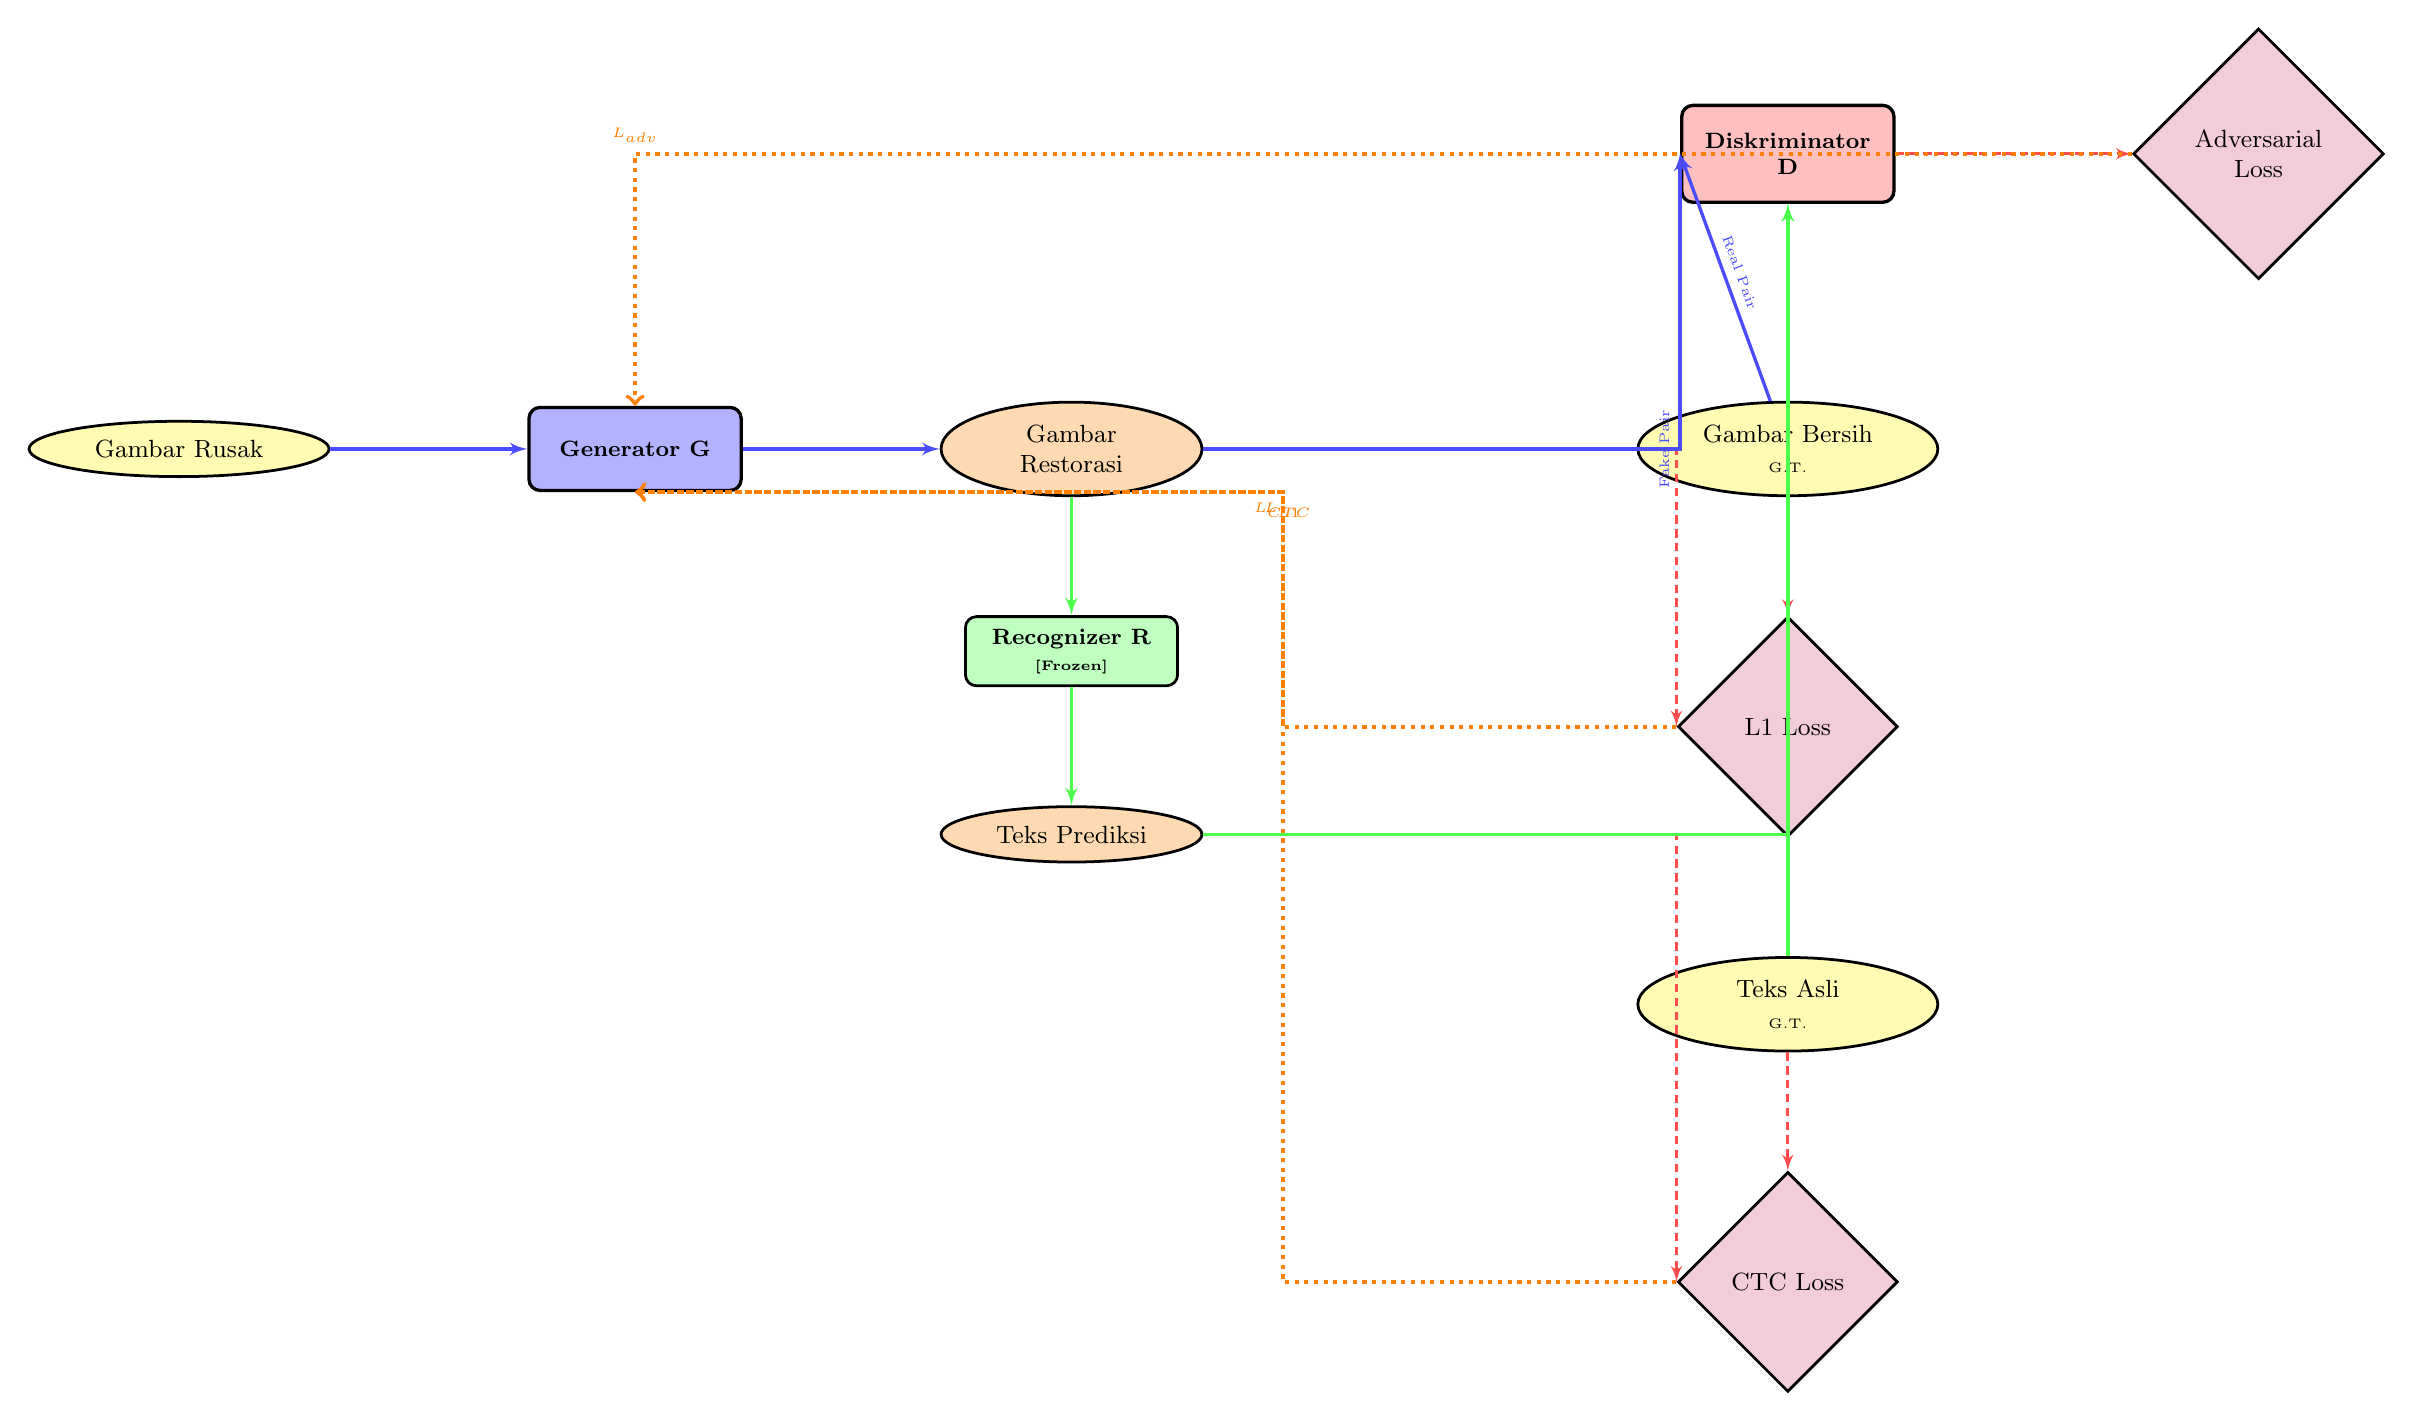
\begin{tikzpicture}[
        node distance=1.5cm and 1.5cm,
        auto,
        thick,
        % STYLES
        generator/.style = {rectangle, draw, fill=blue!30, text width=7em, text centered, rounded corners, minimum height=3em, font=\footnotesize\bfseries, line width=1.2pt},
        discriminator/.style = {rectangle, draw, fill=red!25, text width=7em, text centered, rounded corners, minimum height=3.5em, font=\footnotesize\bfseries, line width=1.2pt},
        recognizer/.style = {rectangle, draw, fill=green!25, text width=7em, text centered, rounded corners, minimum height=2.5em, font=\footnotesize\bfseries, line width=1pt},
        input/.style = {ellipse, draw, fill=yellow!30, text width=7em, text centered, minimum height=2em, font=\small, line width=1pt},
        output/.style = {ellipse, draw, fill=orange!30, text width=6em, text centered, minimum height=2em, font=\small, line width=1pt},
        loss/.style = {diamond, draw, fill=purple!20, text width=6em, text centered, minimum height=2em, font=\small, line width=1pt},
        mainflow/.style = {draw, -latex', line width=1.2pt, color=blue!70},
        lossflow/.style = {draw, -latex', line width=1pt, color=red!70, densely dashed},
        textflow/.style = {draw, -latex', line width=1.2pt, color=green!70},
        feedbackflow/.style = {draw, ->, dotted, line width=1.5pt, color=orange}
    ]
        % --- NODES ---
        % Layer 1: Main Path
        \node [input] (degraded) {Gambar Rusak};
        \node [generator, right=of degraded, xshift=1cm] (generator) {Generator G};
        \node [output, right=of generator, xshift=1cm] (restored) {Gambar Restorasi};
    
        % Layer 2: HTR Path
        \node [recognizer, below=of restored] (recognizer) {Recognizer R \\{\tiny [Frozen]}};
        \node [output, below=of recognizer] (pred_text) {Teks Prediksi};
    
        % Layer 3: Ground Truth & Loss
        \node [input, right=of restored, xshift=4cm] (clean) {Gambar Bersih \\{\tiny G.T.}};
        \node [loss, below=of clean] (l1_loss) {L1 Loss};
        \node [input, below=of l1_loss] (gt_text) {Teks Asli \\{\tiny G.T.}};
        \node [loss, below=of gt_text] (ctc_loss) {CTC Loss};
    
        % Layer 4: Discriminator & Adv Loss
        \node [discriminator, above=of clean, yshift=1cm] (discriminator) {Diskriminator D};
        \node [loss, right=of discriminator, xshift=1.5cm] (adv_loss) {Adversarial Loss};
    
        % --- PATHS ---
        % Main forward flow
        \path [mainflow] (degraded) -- (generator);
        \path [mainflow] (generator) -- (restored);
        \path [textflow] (restored) -- (recognizer);
        \path [textflow] (recognizer) -- (pred_text);
    
        % Loss calculation flows (ACCURATE AND CLEAR)
        \path [lossflow] (restored) -| (l1_loss.west);
        \path [lossflow] (clean) -- (l1_loss.north);
    
        \path [lossflow] (pred_text) -| (ctc_loss.west);
        \path [lossflow] (gt_text) -- (ctc_loss.north);
    
        % Discriminator flow
        \path [mainflow] (restored) -| node[midway, above, sloped, font=\tiny] {Fake Pair} (discriminator.west);
        \path [textflow] (pred_text) -| (discriminator.south);
        \path [mainflow] (clean) -- node[midway, above, sloped, font=\tiny] {Real Pair} (discriminator.west);
        \path [textflow] (gt_text) -- (discriminator.south);
        \path [lossflow] (discriminator) -- (adv_loss);
    
        % Feedback flows to Generator
        \path [feedbackflow] (l1_loss.west) -- ++(-5,0) |- (generator.south) node[midway, below, font=\tiny] {$L_{L1}$};
        \path [feedbackflow] (ctc_loss.west) -- ++(-5,0) |- (generator.south) node[midway, below, font=\tiny] {$L_{CTC}$};
        \path [feedbackflow] (adv_loss.west) -| (generator.north) node[midway, above, font=\tiny] {$L_{adv}$};
    
    \end{tikzpicture}%
}
\caption{Diagram alur arsitektur GAN yang telah direvisi untuk kejelasan. Diagram ini secara akurat menunjukkan input untuk setiap komponen loss: L1 Loss membandingkan dua gambar, CTC Loss membandingkan dua sekuens teks, dan Adversarial Loss berasal dari Diskriminator.}
\label{fig:arch_overview}
\end{figure}

\subsubsection{Desain Generator} % This will be numbered as 4.2.2 Untuk komponen Generator (G), arsitektur yang dipilih adalah U-Net. Arsitektur ini merupakan standar de-facto untuk berbagai tugas translasi gambar-ke-gambar (image-to-image translation), termasuk restorasi, karena efektivitasnya dalam merekonstruksi detail halus pada gambar output. Struktur U-Net terdiri dari dua jalur utama: jalur kontraksi (encoder) dan jalur ekspansi (decoder), yang dihubungkan oleh \textit{skip connections}, seperti diilustrasikan pada Gambar \ref{fig:unet_arch}.

\begin{itemize}
    \item Jalur Encoder: Berfungsi seperti jaringan konvolusi pada umumnya untuk mengekstraksi fitur dari gambar input. Melalui serangkaian blok konvolusi dan operasi \textit{max-pooling}, resolusi spasial gambar secara bertahap dikurangi (downsampling) sementara kedalaman fitur (jumlah channel) ditingkatkan. Proses ini memungkinkan model untuk menangkap informasi kontekstual dari gambar.

    \item Jalur Decoder: Bertugas untuk merekonstruksi gambar output dari representasi fitur yang telah dipelajari oleh encoder. Melalui serangkaian blok \textit{upsampling} dan konvolusi, resolusi spasial gambar secara bertahap ditingkatkan hingga kembali ke ukuran aslinya.

    \item Skip Connections: Ini adalah fitur utama dari arsitektur U-Net. Koneksi ini menghubungkan secara langsung feature map dari lapisan di jalur encoder ke lapisan yang bersesuaian di jalur decoder. Dengan meneruskan informasi dari lapisan awal (yang kaya akan detail spasial) ke lapisan akhir, U-Net mampu mengatasi hilangnya informasi detail yang sering terjadi pada arsitektur encoder-decoder standar. Untuk tugas restorasi dokumen, ini sangat penting untuk menjaga ketajaman dan keutuhan gurat-gurat tipis pada karakter tulisan tangan.
\end{itemize}
\begin{figure}[H] % Memaksa gambar muncul di sini setelah penjelasan generator
\centering
\resizebox{0.9\textwidth}{!}{%
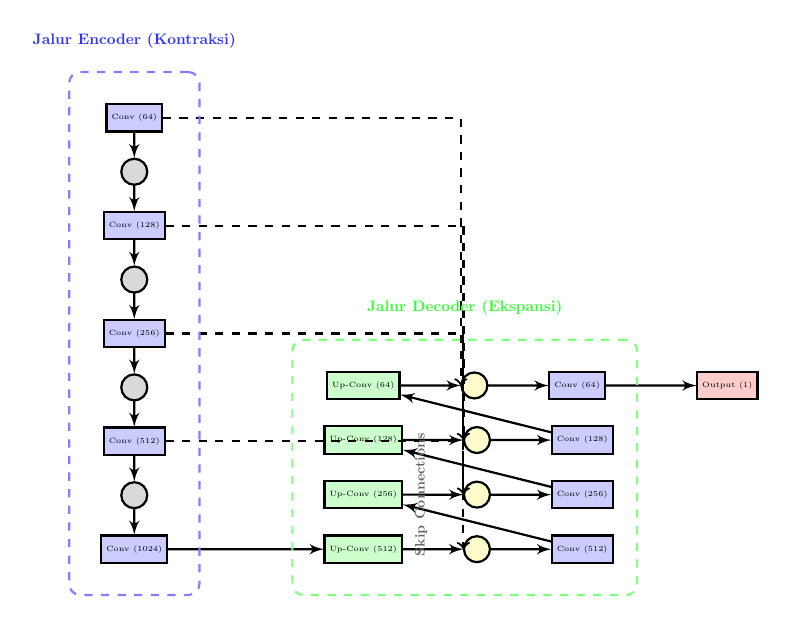
\begin{tikzpicture}[scale=0.55, transform shape, node distance=0.6cm, auto, thick,
    block/.style = {rectangle, draw, fill=blue!20, text centered, minimum height=1.8em, minimum width=3.5em, font=\tiny},
    upconv/.style = {rectangle, draw, fill=green!20, text centered, minimum height=1.8em, minimum width=3.5em, font=\tiny},
    merge/.style = {circle, draw, fill=yellow!20, inner sep=0pt, minimum size=6mm},
    pool/.style = {circle, draw, fill=gray!30, inner sep=0pt, minimum size=6mm},
    output/.style = {rectangle, draw, fill=red!20, text centered, minimum height=1.8em, minimum width=3em, font=\tiny}]

    % Encoder Path
    \node[block] (e1) {Conv (64)};
    \node[pool, below=of e1] (p1) {};
    \node[block, below=of p1] (e2) {Conv (128)};
    \node[pool, below=of e2] (p2) {};
    \node[block, below=of p2] (e3) {Conv (256)};
    \node[pool, below=of e3] (p3) {};
    \node[block, below=of p3] (e4) {Conv (512)};
    \node[pool, below=of e4] (p4) {};

    % Bottleneck
    \node[block, below=of p4] (b) {Conv (1024)};

    % Decoder Path
    \node[upconv, right=of b, xshift=3cm] (u4) {Up-Conv (512)};
    \node[merge, right=of u4, xshift=0.8cm] (m4) {};
    \node[block, right=of m4, xshift=0.8cm] (d4) {Conv (512)};

    \node[upconv, above=of u4] (u3) {Up-Conv (256)};
    \node[merge, right=of u3, xshift=0.8cm] (m3) {};
    \node[block, right=of m3, xshift=0.8cm] (d3) {Conv (256)};

    \node[upconv, above=of u3] (u2) {Up-Conv (128)};
    \node[merge, right=of u2, xshift=0.8cm] (m2) {};
    \node[block, right=of m2, xshift=0.8cm] (d2) {Conv (128)};

    \node[upconv, above=of u2] (u1) {Up-Conv (64)};
    \node[merge, right=of u1, xshift=0.8cm] (m1) {};
    \node[block, right=of m1, xshift=0.8cm] (d1) {Conv (64)};

    \node[output, right=of d1, xshift=1.5cm] (output) {Output (1)};

    % Connections
    \path[line] (e1) -- (p1);
    \path[line] (p1) -- (e2);
    \path[line] (e2) -- (p2);
    \path[line] (p2) -- (e3);
    \path[line] (e3) -- (p3);
    \path[line] (p3) -- (e4);
    \path[line] (e4) -- (p4);
    \path[line] (p4) -- (b);

    \path[line] (b) -- (u4);
    \path[line] (u4) -- (m4);
    \path[line] (m4) -- (d4);

    \path[line] (d4) -- (u3);
    \path[line] (u3) -- (m3);
    \path[line] (m3) -- (d3);

    \path[line] (d3) -- (u2);
    \path[line] (u2) -- (m2);
    \path[line] (m2) -- (d2);

    \path[line] (d2) -- (u1);
    \path[line] (u1) -- (m1);
    \path[line] (m1) -- (d1);

    \path[line] (d1) -- (output);

    % Skip Connections
    \path[skipline] (e4.east) -| (m4.west);
    \path[skipline] (e3.east) -| (m3.west);
    \path[skipline] (e2.east) -| (m2.west);
    \path[skipline] (e1.east) -| (m1.west);

    % --- NEW LABELS ---
    % Bounding box for Encoder
    \node[draw=blue!50, thick, dashed, rounded corners, inner sep=0.4cm, fit=(e1) (p4) (b), label={[blue!80, yshift=0.4cm]above:\textbf{Jalur Encoder (Kontraksi)}}] {};
    % Bounding box for Decoder
    \node[draw=green!50, thick, dashed, rounded corners, inner sep=0.4cm, fit=(u4) (d1), label={[green!80, yshift=0.4cm]above:\textbf{Jalur Decoder (Ekspansi)}}] {};
    % Label for Skip Connections
    \node[font=\small\bfseries, text=black!60, rotate=90, anchor=south] at ($(m3.west) - (0.7, 0)$) {Skip Connections};
\end{tikzpicture}%
}% end resizebox
\caption{Diagram arsitektur U-Net yang digunakan sebagai Generator.}
\label{fig:unet_arch}
\end{figure}

\subsubsection{Desain Recognizer} % This will be numbered as 4.2.3
Komponen Recognizer (R) memainkan peran khusus dan esensial dalam arsitektur yang diusulkan. Berbeda dengan komponen lain, Recognizer tidak dilatih selama proses training GAN. Sebaliknya, komponen ini merupakan sebuah model Handwritten Text Recognition (HTR) berbasis Transformer yang telah dilatih sebelumnya (\textit{pre-trained}) dan bobotnya dibekukan (\textit{frozen}) atau diatur sebagai \textit{non-trainable}.

\paragraph{Fungsi Utama dan Peran dalam Arsitektur}

Recognizer berfungsi sebagai evaluator keterbacaan teks yang objektif. Komponen ini menerima gambar hasil restorasi dari Generator dan menghasilkan distribusi probabilitas karakter untuk mengukur keterbacaan hasil restorasi. Output dari Recognizer digunakan untuk dua tujuan:

\begin{enumerate}[nosep]
    \item Sebagai input teks untuk Diskriminator, yang menilai koherensi antara gambar dan teks yang dikenali.
    \item Sebagai input untuk kalkulasi CTC Loss, yang secara langsung mengukur seberapa dapat dibaca gambar hasil restorasi.
\end{enumerate}

\paragraph{Arsitektur High-Level}

Recognizer menggunakan arsitektur CNN+Transformer yang dirancang khusus untuk dokumen kuno:

\begin{itemize}
    \item \textbf{CNN Backbone:} Mengekstrak fitur visual hierarkis dari stroke dasar hingga kompleksitas karakter
    \item \textbf{Transformer Encoder:} Menangkap dependensi jarak jauh dan konteks linguistik dengan multi-head attention
    \item \textbf{CTC Output Layer:} Menghasilkan probabilitas karakter untuk setiap timestep
\end{itemize}

Detail justifikasi pemilihan arsitektur CNN+Transformer untuk kasus paleografi telah dibahas secara komprehensif pada Bab 2.3.4.

\subsubsection{Desain Diskriminator Dual-Modal} % This will be numbered as 4.2.4

Inovasi utama dalam rancangan solusi ini terletak pada arsitektur Diskriminator (D). Berbeda dengan diskriminator pada GAN konvensional yang hanya menilai realisme sebuah gambar (unimodal), diskriminator yang diusulkan bersifat \textbf{dual-modal}. Tujuannya tidak hanya untuk membedakan gambar asli dari gambar palsu, tetapi juga untuk menilai \textbf{koherensi} antara konten visual sebuah gambar dengan konten semantik dari teks yang diekstraksi dari gambar tersebut.

Diskriminator ini menerima sepasang input: sebuah gambar dan sebuah representasi teks. Tugasnya adalah menghasilkan skor probabilitas tunggal yang menyatakan apakah pasangan tersebut adalah pasangan \textit{(gambar bersih, teks asli)} yang koheren, atau pasangan \textit{(gambar restorasi, teks prediksi)} yang kemungkinan besar tidak koheren.

Arsitektur ini terdiri dari dua jalur pemrosesan paralel yang kemudian digabungkan:

\begin{itemize}
    \item \textbf{Jalur Input Gambar:} Serangkaian lapisan Conv2D dengan LeakyReLU dan BatchNormalization untuk mengekstrak fitur visual
    \item \textbf{Jalur Input Teks:} Layer Embedding dan LSTM untuk memproses representasi teks dan menangkap konteks
    \item \textbf{Fusi dan Klasifikasi:} Konkatenasi fitur visual dan tekstual, diikuti Dense layers untuk klasifikasi akhir
\end{itemize}

\subsubsection{Desain Fungsi Loss} % This will be numbered as 4.2.5

Optimalisasi arsitektur GAN yang diusulkan mengandalkan dua fungsi loss yang bekerja secara simultan. Desain fungsi loss untuk Generator menjadi salah satu kontribusi utama karena secara eksplisit memasukkan metrik keterbacaan teks.

\paragraph{Fungsi Loss Diskriminator}
Fungsi loss untuk Diskriminator ($L_D$) menggunakan Binary Cross-Entropy (BCE) standar untuk membedakan pasangan data asli dan palsu:

\begin{equation}
L_D = -\mathbb{E}_{x,y}[\log D(x, y)] - \mathbb{E}_{z,y^{\prime}}[\log(1 - D(G(z), y^{\prime}))]
\end{equation}

\paragraph{Fungsi Loss Generator}
Fungsi loss untuk Generator ($L_G$) dirancang untuk mencapai dua tujuan: menghasilkan gambar realistis dan gambar yang teksnya dapat dibaca dengan baik. $L_G$ disusun sebagai kombinasi tiga komponen loss:

\subparagraph{1. Adversarial Loss ($L_{adv}$)}
Mengukur kemampuan Generator dalam "menipu" Diskriminator:
\begin{equation}
L_{adv} = -\mathbb{E}_{z,y^{\prime}}[\log D(G(z), y^{\prime})]
\end{equation}

\subparagraph{2. Reconstruction Loss ($L_{L1}$)}
L1 Loss untuk kemiripan piksel dengan ground truth:
\begin{equation}
L_{L1} = \mathbb{E}_{x,G(z)}[\|x - G(z)\|_1]
\end{equation}

\subparagraph{3. CTC Readability Loss ($L_{CTC}$)}
Inovasi kunci: CTC loss dari frozen HTR model untuk mengoptimalkan keterbacaan teks:
\begin{equation}
L_{CTC} = \mathbb{E}_{z,t}[\text{CTC}(R(G(z)), t)]
\end{equation}

\paragraph{Fungsi Loss Gabungan}
Ketiga komponen loss tersebut digabungkan menjadi satu fungsi loss total untuk Generator:
\begin{equation}
L_G = \lambda_{adv} L_{adv} + \lambda_{L1} L_{L1} + \lambda_{CTC} L_{CTC}
\end{equation}
Bobot $\lambda_{adv}$, $\lambda_{L1}$, dan $\lambda_{CTC}$ adalah hyperparameter yang dapat disesuaikan untuk menyeimbangkan kontribusi dari setiap komponen loss terhadap proses training Generator.

\section{KESIMPULAN DAN REKOMENDASI}
\label{sec:kesimpulan}

Berdasarkan analisis kebutuhan sistem dan rancangan arsitektur yang telah diuraikan, bab ini telah menyajikan desain komprehensif untuk framework GAN-HTR yang mampu melakukan restorasi dokumen terdegradasi dengan orientasi pada keterbacaan teks. Rancangan solusi ini memenuhi semua kebutuhan fungsional dan non-fungsional yang telah diidentifikasi, dengan memberikan perhatian khusus pada keseimbangan antara kualitas visual dan keterbacaan tekstual.

\subsection{Kesimpulan Desain}

\paragraph{Analisis Kebutuhan Sistem}
Telah diidentifikasi total 12 kebutuhan sistem yang terdiri dari 8 kebutuhan fungsional dan 4 kebutuhan non-fungsional. Kebutuhan-kebutuhan ini mencakup aspek kemampuan restorasi visual, penanganan berbagai jenis degradasi, integrasi dengan HTR, pemrosesan batch, dukungan dataset sintetis, format output yang terdefinisi, fleksibilitas input, kapabilitas integrasi sistem, serta target performa untuk kualitas visual, keterbacaan teks, efisiensi waktu, dan reproduktifitas.

\paragraph{Rancangan Arsitektur}
Arsitektur yang diusulkan terdiri dari tiga komponen utama yang berinteraksi dalam kerangka kerja adversarial:

\begin{enumerate}
    \item \textbf{Generator (U-Net):} Menerima gambar dokumen terdegradasi dan menghasilkan versi restorasi dengan mempertahankan detail teks melalui skip connections.

    \item \textbf{Recognizer (Transformer-based HTR):} Model beku yang berfungsi sebagai evaluator keterbacaan teks yang objektif dan konsisten.

    \item \textbf{Diskriminator Dual-Modal:} Menggabungkan evaluasi visual dan tekstual untuk memastikan hasil restorasi tidak hanya realistis secara visual tetapi juga koheren secara tekstual.
\end{enumerate}

\paragraph{Fungsi Loss Multi-Komponen}
Fungsi loss gabungan yang mengintegrasikan adversarial loss, L1 reconstruction loss, dan CTC readability loss memberikan optimasi yang seimbang antara kualitas visual dan keterbacaan teks, yang merupakan inovasi kunci dari penelitian ini.

\subsection{Rekomendasi Implementasi}

Detail implementasi teknis dari rancangan arsitektur ini telah dipindahkan ke Bab 3 (Metodologi Penelitian) pada bagian 3.3.2 "Detail Implementasi Framework". Implementasi mencakup lingkungan eksperimen, pipeline persiapan dataset, konfigurasi training dan hyperparameter, serta sistem evaluasi komprehensif.

Rekomendasi utama untuk implementasi adalah:
\begin{itemize}
    \item Menggunakan pure FP32 precision untuk stabilitas numerik
    \item Menerapkan gradient clipping dengan clipnorm=1.0
    \item Menggunakan bobot loss yang seimbang ($\lambda_{adv}=1.0$, $\lambda_{L1}=100.0$, $\lambda_{CTC}=1.0$)
    \item Monitor multiple metrics (PSNR, SSIM, CER, WER) untuk evaluasi holistik
\end{itemize}

\subsection{Kontribusi Desain}

Rancangan solusi ini memberikan kontribusi pada:

\begin{enumerate}
    \item \textbf{Inovasi Arsitektural:} Pengembangan Dual Modal Discriminator yang secara eksplisit mengevaluasi koherensi visual-teksual.

    \item \textbf{Integrasi HTR-GAN:} Pendekatan inovatif untuk mengintegrasikan CTC loss dari frozen HTR model ke dalam GAN training.

    \item \textbf{Optimasi Ganda:} Fungsi loss multi-komponen yang menyeimbangkan antara realism visual dan keterbacaan teks.

    \item \textbf{Metodologi End-to-End:} Pipeline lengkap dari persiapan dataset hingga evaluasi yang terdokumentasi dengan baik.
\end{enumerate}

Desain ini memberikan fondasi yang kuat untuk implementasi framework GAN-HTR yang dapat mengatasi tantangan restorasi dokumen historis dengan berorientasi pada peningkatan keterbacaan teks, bukan hanya perbaikan visual semata.

\end{document}
